\chapter{Trunk and Lower Limb Exoskeleton for Stable Autonomous Walking (ETMICAE)}

\section{Description}

The ETMICAE is a bipedal trunk and lower limb exoskeleton to assist the walking movement of people with motor disabilities. It allows the use of the exoskeleton for people that cannot mantain a full control of the body and lower limbs. It includes human gait stability control.

It is currently being developed at the Biomechatronics Laboratory - Mechanical Engineering and Mechanical Systems Department - Politechnic School of the University of São Paulo (USP). This project is being developed in collaboration with the Rehabilitation Medicine Institute of the Clinics Hospital - Medicine School of USP, São Carlos School of Engineering (EESC-USP).

When the project is completed it will mainly contribute in two major areas: Clinical studies and technological studies. For clinical studies, the ETMICAE will be transfered to a clinic to test and evaluate the exoskeleton on test subjects with motor disabilities. For the technological studies, the exoskeleton will act as platform for testing of mechanical, electrical and control technologies developed at the Biomechatronics laboratory. 

\section{Mechanical Structure}

The author of this thesis was responsible in designing the hip, thigh, knee and leg mechanical structure, as well as its coupling components. The explanation of this design is described in this section.

\subsection{Hip}

\subsubsection{Description}

The hip of the exoskeleton will have four degrees of freedom, being the abduction/adduction and flexion/extension of both thighs. The exoskeleton will not have the pronation/supination movement of the thighs.

The hips are composed of the following parts:

A base will will attach the hip of the exoskeleton to the support of the motors, located at the back of the user.

\begin{figure}[thpb]
      \centering
      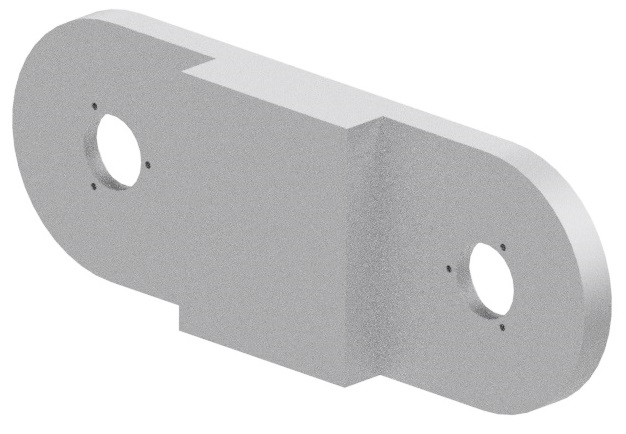
\includegraphics[width=0.4\textwidth]{Images/Base.jpg}
      \caption{Base}
      \label{Base}
   \end{figure}
   
Attached to the base there are two joints that will perform the abduction/adduction degree of freedom for the thighs. For this coupling a shaft supported by two ball bearings will allow the relative movement between the two parts. Between the thigh component and the base, a low friction thrust washer is inserted to support the axial forces and allow smooth slipping. Another thrust washer is positioned at the external part of the joint to, in conjunction with an aluminum cover, support the axial forces.

\begin{figure}[thpb]
      \centering
      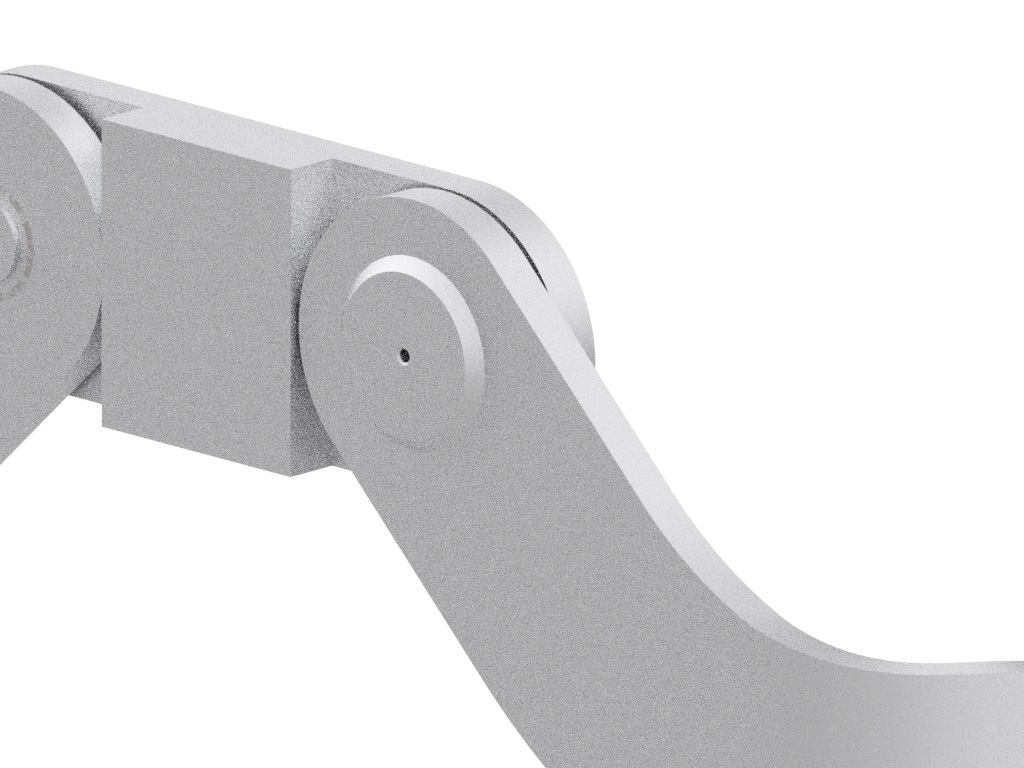
\includegraphics[width=0.4\textwidth]{Images/Junta_quadril_1.jpg}
      \caption{Hip abduction/adduction joint}
      \label{Junta Quadril 1}
   \end{figure}
   
Linked to these joint, a folded aluminum plate extends to the next hip joint.

\begin{figure}[thpb]
      \centering
      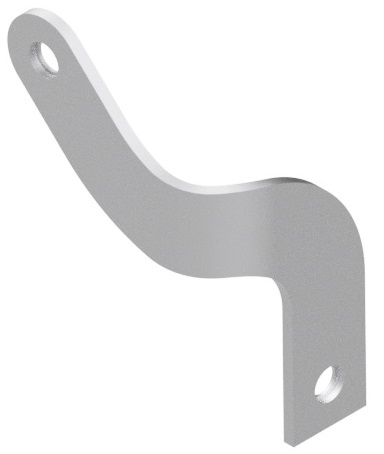
\includegraphics[width=0.4\textwidth]{Images/Chapa_quadril.jpg}
      \caption{Hip plate}
      \label{Chapa Quadril}
   \end{figure}
   
   The lateral joint allows for the flexion/extension degree of freedom of the thighs. This joint is also composed by a shaft supported by two ball bearings with a thrust washer between the two parts.
   
   \begin{figure}[thpb]
      \centering
      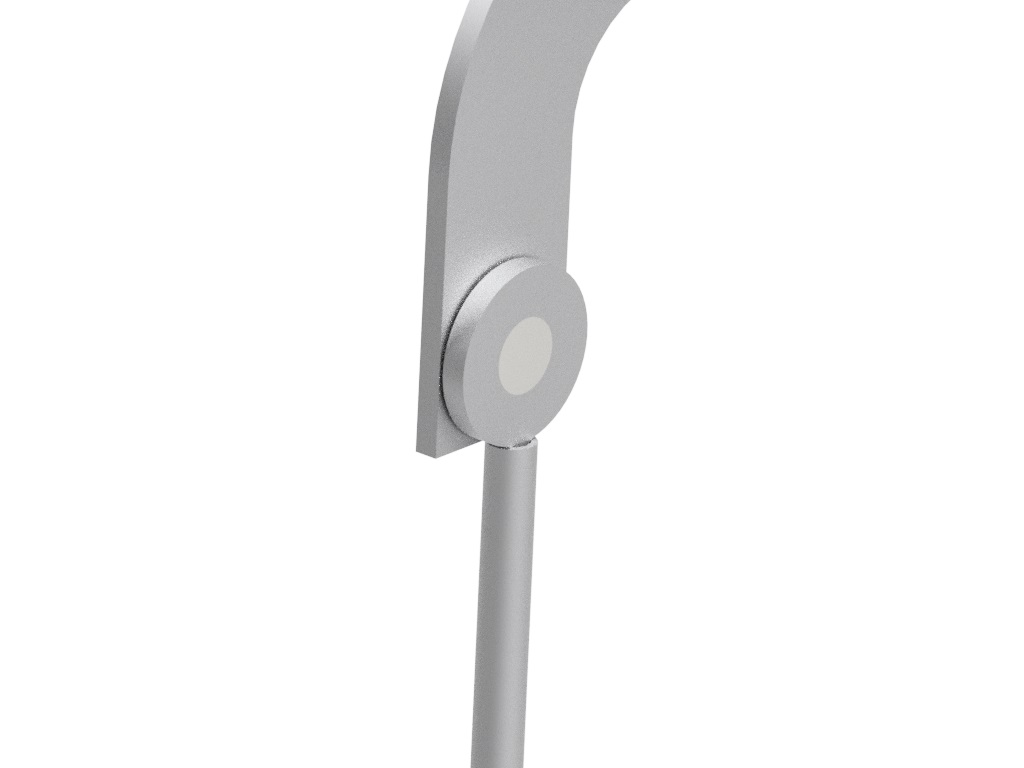
\includegraphics[width=0.5\textwidth]{Images/Junta_Quadril_2.jpg}
      \caption{Hip flexion/extension joint}
      \label{Junta Quadril 2}
   \end{figure}
   
   \subsubsection{Applied Forces}
   
   The weight of the user will be applied at the back support, attached to the hip base. For design purposes, the maximum user weight will be 1000 N. When walking with the exoskeleton, there is the possibility of the user tilting forward his upper body. The torque applied to the hip base due to this misalignment between the upper body and the base is considered as a 25 Nm torque. The torque applied at the joints is equal to 2000 N that is the maximum torque applied by the motors to the joints.
   
      \begin{figure}[thpb]
      \centering
      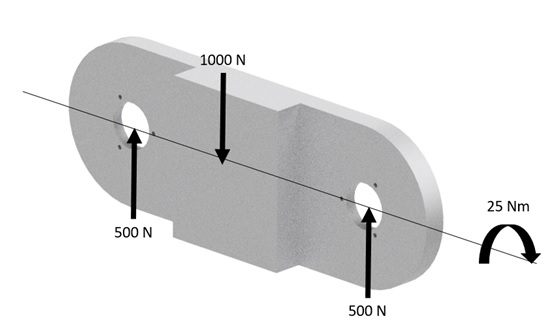
\includegraphics[width=0.4\textwidth]{Images/base_forcas.jpg}
      \caption{Acting forces on the base}
      \label{base forcas}
   \end{figure}
   
   \begin{figure}[b]
      \centering
      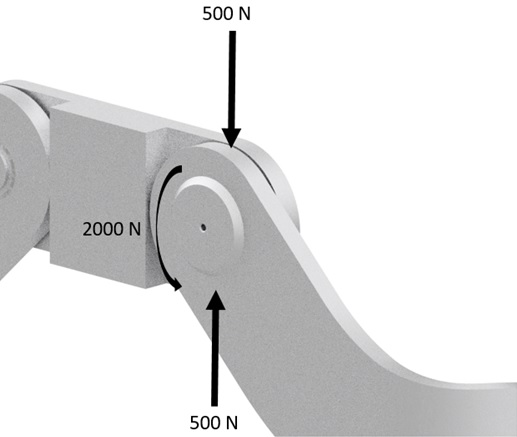
\includegraphics[width=0.4\textwidth]{Images/junta_quadril_1_forcas.jpg}
      \caption{Acting forces on the abduction/adduction joint}
      \label{junta quadril 1 forcas}
   \end{figure}
   

   
   \subsubsection{Materials}
   
   Aluminum was chosen for the structural plates as well as for the joints due to its low weight and high resistance/weight coefficient.
   
   The shafts will be constituted of steel, since they will support high loads. Because of its low dimensions, it is not critical the usage of low weight materials.
   
      \begin{figure}[thpb]
      \centering
      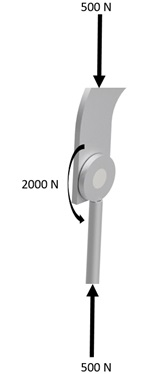
\includegraphics[scale=0.7]{Images/junta_quadril_2_forcas.jpg}
      \caption{Acting forces on the flexion/extension joint}
      \label{junta quadril 2 forcas}
   \end{figure}
   
   For the coupling of the shafts, ball bearings will be used so that the joints can rotate with low friction coefficient, as well as being capable of enduring the high loads applied. The chosen ball bearings were DIN 652 SKF with 2 RS1.
   
   To avoid interference between the two parts of the joints, a Permaglide\textsuperscript{\textregistered} thrust washer model PAW 26 will be used. This thrust washer has the necessary resistance to withstand the applied loads. Also, it is low weight and easier to assemble compared to axial bearings.
   
   The cover attached to the shaft will be made of aluminum.
   
   \bigskip
   
   \subsubsection{Calculations and simulations}
   
   Permaglide\textsuperscript{\textregistered} PAW 26 Thrust Washer:
   
   Torque at the hip due to the misalignment between the upper body and the rotation axis of the hip is considered as a 25 Nm torque. This torque will be supported by the thrust washer. That way:
   
   \begin{equation}
   M = 2\cdot F\cdot\frac{\frac{D_e}{2}+\frac{D_i}{2}}{2}
   \end{equation}
   
   \begin{equation}
   A = \frac{\frac{\pi}{4}(D_e^2-D_i^2)}{2}
   \end{equation}
   
   \begin{equation}
   \sigma = \frac{F}{A}
   \end{equation}
   
   Where M is the torque applied to the hip, F is the reaction force in the thrust washer and cover of the joint, $D_e$ and $D_i$ are the external and internal diameter of the thrust washer, respectively, A is the thrust washer area that will support the load and $\sigma$ is the load.
   
   Resulting in:
   
   $$\sigma \cong 1.5 MPa < \sigma_{crit}$$
   
   Therefore, the PAW 26 thrust washer is suitable to be used.
   
   DIN 625 SKF with 2 RS1 (SKF 61902-2RS1) ball bearing:
   
   Chosen through the SKF\textsuperscript{TM} bearing selection tool, for a load equal to 500 N and lifespan of 10000 hours. The tool can be found at: http://www.skf.com/group/knowledge-centre/engineering-tools/skfbearingselect.html
   
   All components were numerically simulated at the Autodesk\textsuperscript{TM} Inventor 2017 software. 
   
   \begin{figure}[thpb]
      \centering
      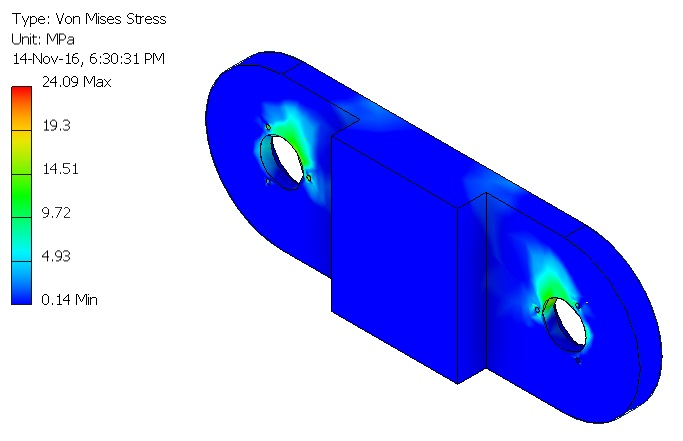
\includegraphics[scale=0.6]{Images/Simulacao_Base.jpg}
      \caption{Numerical simulation of the base}
      \label{simulacao base}
   \end{figure}
   
   \begin{figure}[thpb]
      \centering
      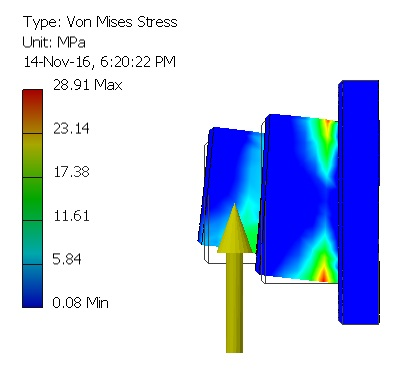
\includegraphics[scale=0.8]{Images/Simulacao_eixo.jpg}
      \caption{Numerical simulation of the joint shafts}
      \label{simulacao eixo}
   \end{figure}
   
   \begin{figure}[thpb]
      \centering
      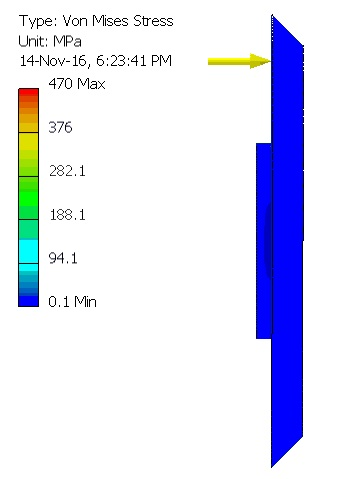
\includegraphics[scale=0.6]{Images/Simulacao_tampa.jpg}
      \caption{Numerical simulation of the cover}
      \label{simulacao tampa}
   \end{figure}
   
   \subsection{Knee}
   
   \subsubsection{Description}
   
   Each knee will have only one degree of freedom, aligned to the flexion/extension joint of the user. It is constituted of the following parts:
   
   A bar that extends from the flexion/extension joint of the hip to the knee joint. This bar stays parallel to the user's thigh.
   
   \begin{figure}[thpb]
      \centering
      
      \begin{subfigure}[b]{0.45\textwidth}
      	\centering
      	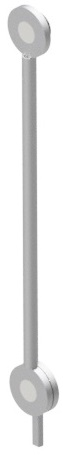
\includegraphics[height=0.3\textheight]{Images/Barra_Coxa.jpg}
      	\caption{Thigh}
      	\label{barra coxa}  
      \end{subfigure}
      ~
      \begin{subfigure}[b]{0.45\textwidth}
      	\centering
      	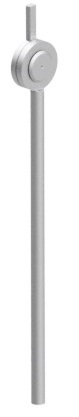
\includegraphics[height=0.3\textheight]{Images/Canela.jpg}
     	\caption{Leg}
     	\label{barra canela}
      \end{subfigure}
      \caption{Thigh and leg bars}
      
   \end{figure}
   
   Attached to the thigh bar, a rotation joint allows the flexion/extension movement of the mechanism. At this joint a shaft supported by two ball bearings will be used. Between the two parts of the joint a low friction coefficient thrust washer is positioned to support the axial forces and allow for smooth sliding between the parts. Another thrust washer is positioned at the external part of the joint, along with a metallic cover, to support the axial forces.
   
   \begin{figure}[thpb]
      \centering
      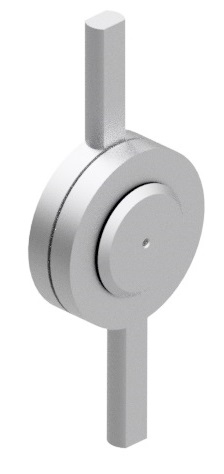
\includegraphics[scale=0.5]{Images/Junta_Joelho.jpg}
      \caption{Knee flexion/extension joint}
      \label{junta joelho}
   \end{figure}
   
   Attached to this joint, another metallic bar extends to the ankle.
   
   
   \subsubsection{Applied forces}
   
   The forces applied at the knee joint are the torque that the motor applies at the joint and the weight of the user and exoskeleton. 
   
   \begin{figure}[thpb]
      \centering
      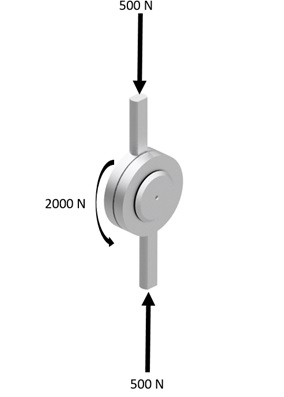
\includegraphics[scale=0.5]{Images/joelho_forcas.jpg}
      \caption{Forces applied to the knee joint}
      \label{joelho forcas}
   \end{figure}
   
   \subsubsection{Materials}
   
   Aluminum is the metal constituting the joints. This material was chosen for its low weight and high resistance/weight coefficient.
   
   For the bars, steel bars will be used for its high resistance and easy acquisition.
   
   For the same reasons stated at the hip, the shafts will be made of steel.
   
   Like before, DIN 625 SKF with 2 RS1 ball bearings and PAW 26 Permaglide\textsuperscript{\textregistered} thrust washers will be used.
   
   \subsubsection{Calculations and simulations}
   
   \begin{figure}[thpb]
      \centering
      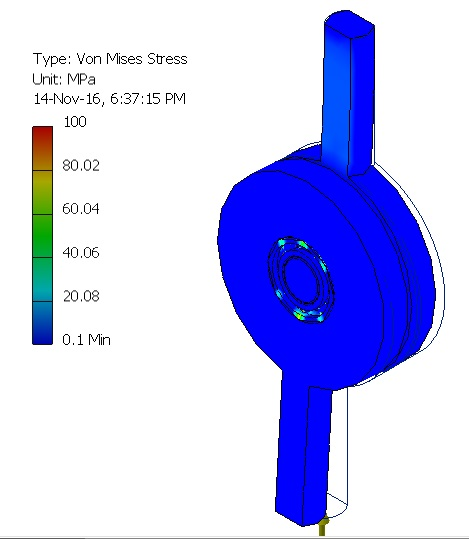
\includegraphics[scale=0.5]{Images/Simulacao_Joelho.jpg}
      \caption{Numerical simulation of the knee joint}
      \label{simulacao joelho}
   \end{figure}
   
